\section{Implementation}
\label{section:implementation}

%Application of Singular Value Decomposition to FEM results compression

The objective of the compression algorithm is to reduce amount of data representing FEM results and also the ability to reconstruct original data from its smaller representation. This saves storage capacity and also accelerates data transfer between computers as the analysis itself and the post-processing of results is usually done on different work stations.

Compression method can be lossy or lossless based on quality of data reconstructed of its compressed representation. Lossless methods are able to fully recreate original data. Lossy methods on the other hand produce only approximations of original data. 

SVD is used as part of the compression algorithm. SVD method applied to arbitrary matrix produces decomposition that consist of corresponding singular values and singular vectors. This process is fully reversible (with the assumption that the numerical errors are negligible). The original matrix can be reconstructed by the multiplication of decomposed parts. However, compression algorithm modifies decomposition to create low-rank approximation of the matrix. The reconstructed matrix slightly differs from the original matrix and algorithm therefore does lossy compression.

To 
% jak ziskam matici na kterou aplikuji SVD? popsat z ceho se skladaji fem data a jak se naskladaji do matice


%A= U1*S1 *V1T + U2*S2*V2T…………Un* S n*Vn T

%Ar = U1*S1 *V1T + U2* S 2*V2T…………Un* Sr*VrT

% vlozit obrazek svd dekompozice z prezentace
\begin{figure}[ht]
\centering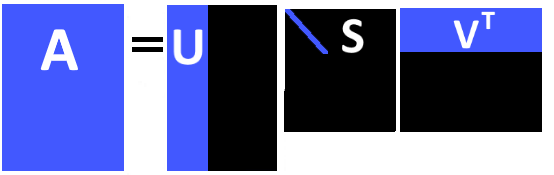
\includegraphics[width=0.7\textwidth]{figures/low_rank_decomposition_diagram}
\caption{Decomposition of input matrix $\mtrx{A}$ into diagonal matrix of singular values $\mtrx{\Sigma}$ and matrices of left and right singular vectors}
\label{fig:lowrank_svd}
\end{figure}

% jak se pocita chyba; jak se da ridit maximalni chyba

\subsection{Algorithm description}

% computational complexity; algorithm steps ...

\subsection{Encoding of data}
%converting to text representation, base64, NaN, ...
\subsection{Optimization}
%At first: algorithm complexity, table with execution times...
% Randomized SVD, Parallelization, Sparse matrix of details